\chapter{Laufzeitsicht}
\label{ch:Laufzeitsicht}

Szenario: Daten Werden übergeben und dann simuliert
\begin{figure}[tbh]
    \centering
    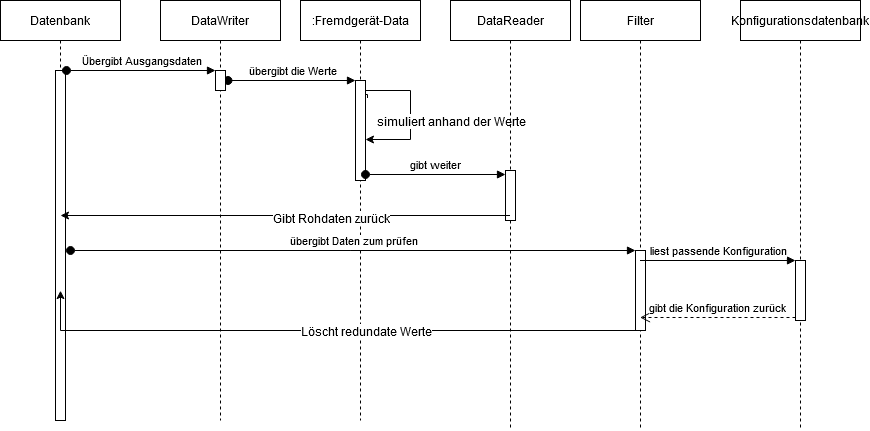
\includegraphics[width=0.7\textwidth]{Graphics/Laufzeit_Rohdaten.png}
    \caption{Laufzeitsicht für Rohdaten}
    \label{fig:LaufzeitRohdaten}
  \end{figure}

  Szenario: Daten werden gefiltert
\begin{figure}[tbh]
    \centering
    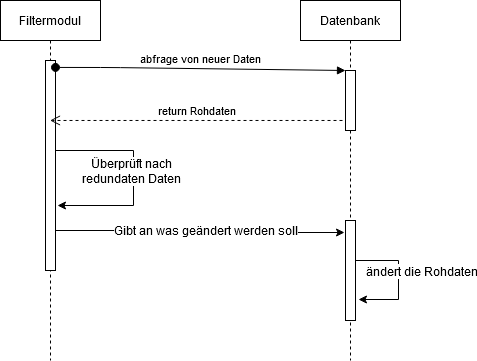
\includegraphics[width=0.7\textwidth]{Graphics/Laufzeit_Filter.png}
    \caption{Laufzeitsicht für Filter}
    \label{fig:LaufzeitFilter}
  \end{figure}